\documentclass[12pt]{article}
\usepackage{geometry}
\geometry{a4paper}


\usepackage{color}
\usepackage{hyperref}
\usepackage{amsmath}
\usepackage{amsfonts}
\usepackage{amssymb}
\usepackage{graphicx}
\usepackage{tcolorbox}
\usepackage{listings}
\usepackage{here}
\usepackage{txfonts}
\usepackage{algorithm}
\usepackage{algorithmic}
\usepackage{siunitx}
\usepackage{xcolor}
\usepackage{ascmac}
%\usepackage{fancybx}

\lstset {language = c++,
  basicstyle = \ttfamily \scriptsize,
  commentstyle = \textit,
  frame = tRBl,
  framesep = 5pt,
  showstringspaces = false,
  numbers = left,
  stepnumber = 1,
  numberstyle = \tiny,
  tabsize = 2,
  keywordstyle = \bfseries \color{blue},
  stringstyle=\color{magenta},
  commentstyle=\color{red},
  morecomment=[l][\color{red}]{\#}
  showstringspaces=false, % don't mark spaces in strings
}
\newcommand{\bi}[1]{\mathbf{#1}}
\newcommand{\bs}[1]{\boldsymbol{#1}}  % bold for greek characters
\newcommand{\bbR}{\mathbb{R}}

\author{Nobuyuki Umetani}

\title{Finite Element Method:\\ Diffusion Equation}
\author{Nobuyuki Umetani}

\begin{document}
\maketitle
\tableofcontents


%CENTER: Solving method of thermal diffusion equation by finite element method
%CENTER: file: diffusion_3d.gif file: move_diffusion_test.gif


\section{Table of Contents}

\section{Overview}

We describe a method of finite element method analysis of thermal diffusion equation, which is an equation that heat diffuses with time. First, formulate the thermal diffusion equation, convert it to a weak form, and discretize the finite element method. We will also refer to weak formalization and finite element method discretization in the axisymmetric problem.


\section{Finite Element Formulation}
\subsection{Derivation of Governing Equations}
%
According to the Fourier's law, the heat flow velocity vector $\Phi$ is represented by the gradient of the temperature field $T(x)$ as follows.
%
\begin{equation}
\label{eqn:fouriers_law}
\Phi = -\lambda\nabla T
\end{equation}
%
However, $\lambda$ is a heat conduction coefficient, which is a positive definite symmetric tensor that associates the temperature gradient with the heat flow velocity.
%
On the other hand,
%
\begin{equation}
\label{eqn:heat_conservation}
\rho c \frac{dT}{dt}= -\nabla\cdot\Phi + f
\end{equation}
%
Where $f$ is the calorific value per unit volume.
%
We take the divergence of both sides of \eqref{eqn:fouriers_law} and substitute equation \eqref{eqn:heat_conservation}.
%
\begin{eqnarray}
&&\nabla\cdot\Phi = -\nabla\cdot(\lambda\nabla T)\\        
&\Leftrightarrow& \rho c \frac{dT}{dt} = \nabla\cdot(\lambda\nabla T) + f,
\end{eqnarray}

And a thermal diffusion equation is obtained.

\begin{tcolorbox}[title=Thermal Diffusion Equation]
\begin{equation}
\rho c \frac{dT}{dt} = \nabla\cdot(\lambda\nabla T) + f
\end{equation}
\end{tcolorbox}

$\lambda$ is the tensor quantity, but in the case of isotropic physical properties it can be treated as a scalar quantity because the direction of the temperature gradient and the direction of the heat flow velocity vector coincide. Assuming that the thermal conductivity is constant, it is as follows.

\begin{tcolorbox}[title=Thermal diffusion equation (constant thermal conductivity isotropic)]
\begin{equation}
\rho c \frac{dT}{dt} = \lambda \nabla^2 T + f
\end{equation}
\end{tcolorbox}





\subsection{Weak Formulation}
Expression development is performed assuming that the heat conduction coefficient is isotropic and constant as in Eq. (3).
%
As the boundary conditions, consider the following two.
%
\begin{enumerate}
\item $T=T_1$ is given on the surface area $S_1$
\item The heat inflow amount per unit area $Q$ is given on the surface area $S_2$.
\end{enumerate}

\begin{figure}[hbtp!]
\center
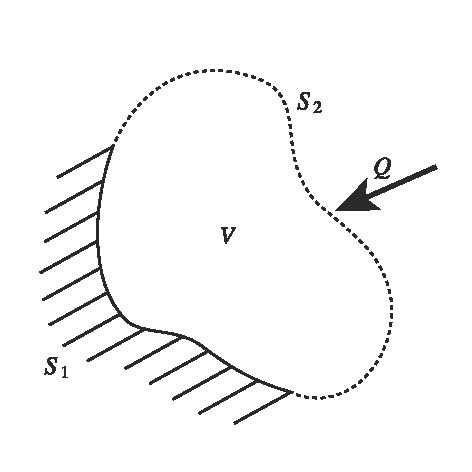
\includegraphics[width=80mm]{images/heat_domain}
\caption{Problem settings}
\end{figure}


From the Fourier's law of Eq. (1)
%
\begin{equation}
Q=\lambda\frac{\partial T}{\partial n}.
\end{equation}

The fact that the inflow amount rather than the outflow amount is given as the boundary condition is in line with the reality that in actual practice it is heated more than the cooling in many cases.
%
(3) are multiplied by an arbitrary virtual variable $\delta T$ which becomes 0 on the fixed boundary $S_1$ on both sides of the equation (3) and integrated over the analysis area $V$, and the Gauss divergence theorem is applied as follows.

\begin{eqnarray}
&&\int_V \rho c \delta T\dot{T} dV = \int_V \delta T\left(\lambda \nabla^2 T + f \right)dV\;\;\;\;\forall\delta T \\      
&\Leftrightarrow& \int_V \rho c \delta T \dot{T} dV= \int_V  \nabla\cdot\left( \lambda\delta T \nabla T\right) - \lambda\nabla\delta T\nabla T+ \delta T f dV\;\;\;\;\forall\delta T\\     
&\Leftrightarrow& \int_V \rho c \delta T\dot{T}  + \lambda\nabla\delta T\nabla TdV= \int_V \delta T f dV + \int_S  \bi{n}\cdot\left( \lambda\delta T \nabla T\right) dS\;\;\;\;\forall\delta T\\    
&\Leftrightarrow& \int_V \rho c \delta T\dot{T}  + \lambda\nabla\delta T\nabla TdV= \int_V \delta T f dV + \int_S  \delta T \lambda\frac{\partial T}{\partial n} dS\;\;\;\;\forall\delta T\\     
&\Leftrightarrow& \int_V \rho c \delta T \dot{T}  + \lambda\nabla\delta T\nabla TdV= \int_V \delta T f dV + \int_S  \delta T Q dS\;\;\;\;\forall\delta T
\end{eqnarray}

\begin{tcolorbox}[title=Heat conduction equation of weak form]
\begin{equation}
\int_V\rho c \delta T\dot{T}  + \lambda\nabla\delta T\nabla TdV= \int_V \delta T f dV + \int_S  \delta T Q dS\;\;\;\;\forall\delta T
\end{equation}
\end{tcolorbox}



\subsection{Finite Element Discretization}
Suppose the region $V$ is meshed. The integral of Eq. (4) can be obtained by summing up all the integral within each element. In other words,
%
\begin{equation}
\sum_e\int_{V_e} \rho c \delta T\dot{T}  + \lambda\nabla\delta T\nabla TdV= \sum_e\int_{V_e} \delta T f dV + \sum_e\int_{S_e}  \delta T Q dS\;\;\;\;\forall\delta T
\end{equation}
%
Here, assuming that the variations are performed by the Galerkin method, let $T$ and $\delta T$ be discretized using the interpolation function $N$ in the element as follows.
$T = N^q T^q$, $\delta T = N^p \delta T^p$
Also assume that the surface of the region is discretized using the interpolation function $\bar{N}$ as follows.

\begin{equation}
\delta T = \bar{N}^p \delta T^p
\end{equation}

Substituting these into Eq. (5), we can derive the element stiffness matrix and the overall stiffness matrix as follows. However, in formula deformation it is assumed that numbering within element $\{p,q\}\rightarrow \{a,b\}$ holds.

\begin{eqnarray}
&&\sum_e\int_{V_e} \rho c N^p\delta T^pN^q\dot{T}^q  + \lambda\nabla N^p\delta T^p\nabla N^qT^qdV\\
&& = \sum_e\int_{V_e} N^p\delta T^p f dV + \sum_e\int_{S_e}  \bar{N}^p\delta T^p Q dS\;\;\;\;\forall\delta T\\      
&\Leftrightarrow& \sum_e\left(\delta T^p\int_{V_e} \rho c N^pN^q dV \dot{T}^q\right)  + \sum_e\left(\delta T^p\int_{V_e}\lambda\nabla N^p\nabla N^qdVT^q\right)\\
&&=\sum_e\left(\delta T^p\int_{V_e} N^p f dV\right) + \sum_e\left(\delta T^p \int_{S_e}  \bar{N}^pQ dS\right)\;\;\;\;\forall\delta T\\      
&\Leftrightarrow&\delta T^a\left(\sum_e M^{pq} \right)\dot{T}^b  + \delta T^a\left(\sum_eA^{pq}\right)T^b=\\
&&\delta T^a\left(\sum_e {F_{in}}^p_e \right) + \delta T^a\left(\sum_e {F_{out}}^p_e \right)\;\;\;\;\forall\delta T\\      
&\Leftrightarrow&\delta T^a M^{ab} \dot{T}^b  + \delta T^a A^{ab}T^b= \delta T^a F_{in}^a  + \delta T^a F_{out}^a \;\;\;\;\forall\delta T\\       
&\Leftrightarrow& M^{ab} \dot{T}^b  + A^{ab}T^b= F_{in}^a  + F_{out}^a\\       
&\Leftrightarrow& \left[M\right] \{\dot{T}\}  + \left[A\right]\{T\}= \{F_{in}\}  + \{F_{out}\}
\end{eqnarray}

Here, $\left[M\right]$, $\left[A\right]$, $\{F_{in}\}$, $\{F_{out}\}$ are the total mass matrix, the total stiffness matrix, the total external force vector (coming from the body force), and the total external force vector (coming from the surface force).
$\left[M\right]=M^{ab}=\sum_e M^{ab}_e$, $\left[A\right]=A^{ab}=\sum_e A^{ab}_e$, $\{F_{in}\}=F_{in}^a=\sum_e {F_{in}}^a_e$, $\{F_{out}\}=F_{out}^a=\sum_e {F_{ou}}^a_e$
It can be seen that these are obtained by adding together the following matrices in element units.


\begin{tcolorbox}[title=Element mass matrix stiffness matrix external force vector]
\begin{eqnarray}
M_e^{pq}&=&\int_{V_e} \rho c N^pN^q dV\\
A_e^{pq}&=&\int_{V_e}\lambda\nabla N^p\nabla N^qdV\\
{F_{in}}_e^p &=& \int_{V_e} N^p f dV\\
{F_{out}}_e^p &=&  \int_{S_e}  \bar{N}^pQ dS
\end{eqnarray}
\end{tcolorbox}

A time evolution solution is obtained by solving simultaneous linear equations relating to the obtained temperature and its time differentiation using an implicit / explicit time integration scheme.




\section{Axisymmetric Problem}
Consider the axially symmetric three-dimensional problem as shown in the following figure, that is, when all shapes, initial conditions, boundary conditions, and physical property values ​​are axisymmetric, the solution is also axisymmetric. In this case, it can be reduced to a two-dimensional problem in the cross section and the cost of three-dimensional analysis can be greatly reduced.


\begin{figure}[hbtb!]
\center
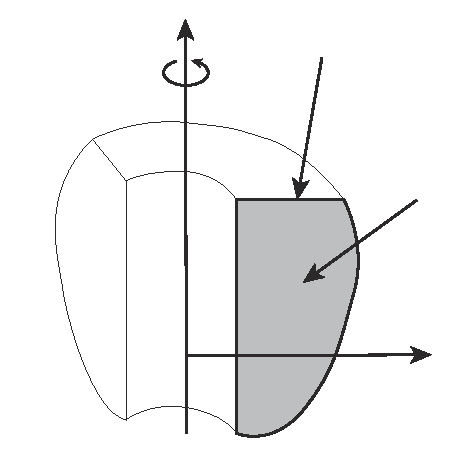
\includegraphics[width=80mm]{images/cylinder_domain.pdf}
\end{figure}




\subsection{Weak Formulation}
%
Discretize the equation (4) two-dimensionally about the cross section in the case of the axisymmetric case. The weak form of the thermal diffusion equation was as follows.

\begin{equation}
\int_V \rho c \delta T\dot{T}  + \lambda\nabla\delta T\nabla TdV= \int_V \delta T f dV + \int_S  \delta T Q dS\;\;\;\;\forall\delta T
\end{equation}

Let's convert the integral variables to $\{x,y,z\}\rightarrow \{r,\theta,z\}$ as follows.

\begin{eqnarray}
\left\{\begin{array}{l}
x\rightarrow r\sin\theta\\ 
y\rightarrow r\cos\theta\\ 
z\rightarrow z\end{array}\right.
\end{eqnarray}

The absolute value of Jacobian in this case is

\begin{eqnarray}
\det J (r,\theta,z)
=
\det \left[\begin{array}{lll}
\sin\theta & r \cos\theta & 0 \\ 
\cos\theta & -r\sin\theta & 0 \\ 
0 & 0 &  1 \end{array}\right] 
= r
\end{eqnarray}

Therefore, it becomes $dxdydz = r drd\theta dz$. Also, as shown in the figure below,

\begin{figure}[htbp!]
\center
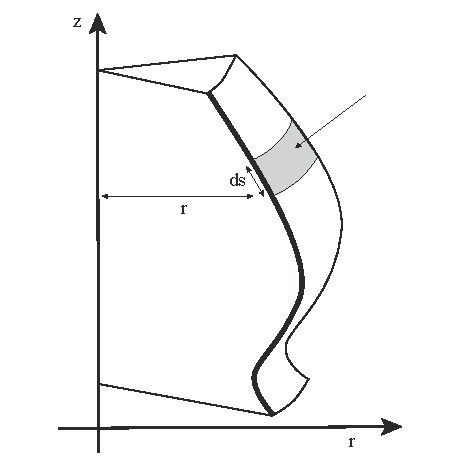
\includegraphics[width=80mm]{images/axis_surface.pdf}
\end{figure}

\begin{equation}
dS = rdsd \theta
\end{equation}

If this is substituted above,

\begin{equation}
\int_\theta\int_r\int_z r\rho c \delta T\dot{T}  + r\lambda\nabla\delta T\nabla T dzdrd\theta = \int_\theta\int_r\int_z \delta T f rdzdrd\theta + \int_\theta \int_s  \delta T Q rdsd\theta\;\;\;\;\forall\delta T
\end{equation}

Since the integrand does not change in the $\theta$ direction, we can remove the integral of $\theta$. Also, if we write $v$ as the two-dimensional integral area of ​​the cross section and $s$ as the boundary of the cross section, weak formalization on the axisymmetric problem as below is obtained.

\begin{tcolorbox}[title=Weak form of thermal diffusion equation for axisymmetric problem]
\begin{equation}
\int_{v_e} r\rho c \delta T\dot{T}  + r \lambda\nabla\delta T\nabla T dv = \int_{v_e} \delta T f rdv + \int_s  \delta T Q rds\;\;\;\;\forall\delta T
\end{equation}
\end{tcolorbox}


\subsection{Finite Element Discretization}
Suppose the region $V$ is meshed. The integral of Eq. (4) can be obtained by summing up all the integral within each element. In other words,
%
\begin{equation}
\sum_e\int_{v_e} r\rho c \delta T\dot{T}  + r\lambda\nabla\delta T\nabla T dv = \sum_e\int_{v_e} \delta T f rdv + \sum_e\int_{s_e}  \delta T Q rds\;\;\;\;\forall\delta T
\end{equation}
%
Here, assuming that the variations are performed by the Galerkin method, it is assumed that $T$ and $\delta T$ are discretized using the interpolation function $N$ in the element as follows.

\begin{align}
T &= N^q T^q\\
\delta T &= N^p \delta T^p
\end{align}


Also assume that the surface of the region is discretized using the interpolation function $\bar{N}$ as follows.

\begin{equation}
\delta T = \bar{N}^p \delta T^p
\end{equation}

Substituting these into Eq. (5), we can derive the element stiffness matrix and the overall stiffness matrix as follows. However, in the formula deformation it is assumed that the numbering within the element $\{p,q\}\rightarrow \{a,b\}$ holds.

\begin{eqnarray}
&&\sum_e\int_{v_e} r\rho c N^p\delta T^pN^q\dot{T}^q  + r\lambda\nabla N^p\delta T^p\nabla N^qT^qdv\\
&&= \sum_e\int_{v_e} rN^p\delta T^p f dv + \sum_e\int_{s_e}  r\bar{N}^p\delta T^p Q ds\;\;\;\;\forall\delta T\\      
&\Leftrightarrow& \sum_e\left(\delta T^p\int_{v_e} r\rho c N^pN^q dV \dot{T}^q dv\right)  + \sum_e\left(\delta T^p\int_{v_e}r\lambda\nabla N^p\nabla N^qdVT^q dv\right)\\
&&\;\;\;\;\;\;\;\;= \sum_e\left(\delta T^p\int_{v_e}r N^p f dv\right) + \sum_e\left(\delta T^p \int_{s_e}r \bar{N}^pQ dS\right)\;\;\;\;\forall\delta T\\ 
&\Leftrightarrow&\delta T^a\left(\sum_e M^{pq} \right)\dot{T}^b  + \delta T^a\left(\sum_eA^{pq}\right)T^b= \delta T^a\left(\sum_e {F_{in}}^p_e \right) + \delta T^a\left(\sum_e {F_{out}}^p_e \right)\;\;\;\;\forall\delta T\\      
&\Leftrightarrow&\delta T^a M^{ab} \dot{T}^b  + \delta T^a A^{ab}T^b= \delta T^a F_{in}^a  + \delta T^a F_{out}^a \;\;\;\;\forall\delta T\\       
&\Leftrightarrow& M^{ab} \dot{T}^b  + A^{ab}T^b= F_{in}^a  + F_{out}^a\\
&\Leftrightarrow& \left[M\right] \{\dot{T}\}  + \left[A\right]\{T\}= \{F_{in}\}  + \{F_{out}\}
\end{eqnarray}

Here, $\left[M\right]$, $\left[A\right]$, $\{F_{in}\}$$\{F_{out}\}$ are the total mass matrix, the total stiffness matrix, the total external force vector (coming from the body force), and the total external force vector (coming from the surface force).

$\left[M\right]=M^{ab}=\sum_e M^{ab}_e$, $\left[A\right]=A^{ab}=\sum_e A^{ab}_e$, $\{F_{in}\}=F_{in}^a=\sum_e {F_{in}}^a_e$, $\{F_{out}\}=F_{out}^a=\sum_e {F_{ou}}^a_e$
It can be seen that these are obtained by adding together the following matrices in element units.


\begin{tcolorbox}[title=Element mass matrix \, stiffness matrix \, external force vector]
\begin{eqnarray}
M_e^{pq}&=&\int_{v_e} r\rho c N^pN^q dv\\
A_e^{pq}&=&\int_{v_e}r\lambda\nabla N^p\nabla N^qdv\\
{F_{in}}_e^p &=& \int_{V_e} rN^p f dv\\
{F_{out}}_e^p &=&  \int_{S_e}  r\bar{N}^pQ ds
\end{eqnarray}
\end{tcolorbox}






\subsection{Derivation of Analytic Element Stiffness Matrix with Lienar Triangle Element}
When interpolation is performed using the linear triangle element, a stiffness matrix can be analytically derived. 
%
A linear interpolation function with such a linear element is expressed by using $L$ instead of $N$.
%
Since the distance $r$ to the axis changes primarily in the triangle

\begin{equation}
r = L^r r^r
\end{equation}

Thus, it can be obtained by interpolating the value of the node. Let's calculate using this.

\begin{equation}
\int_{v_e} (L^1)^a(L^2)^b(L^3)^c dv = \Delta\frac{2!a!b!c!}{(a+b+c+2)!}
\end{equation}

Is used. However, let $\Delta$ be the area of ​​a triangle.



\subsubsection{Element Stiffness Matrix}

\begin{eqnarray}
A_e^{pq}
&=& \int_\Omega L^rr^r\frac{\partial L^p}{\partial r}\frac{\partial  L^q}{\partial r} + L^rr^r\frac{\partial L^p}{\partial z}\frac{\partial L^q}{\partial z} drdz\\
&=& \frac{1}{3}(r^0+r^1+r^2)\left\{\frac{\partial L^p}{\partial r}\frac{\partial  L^q}{\partial r} + \frac{\partial L^p}{\partial z}\frac{\partial L^q}{\partial z} \right\}\Delta
\end{eqnarray}

In the end, in this case, it turns out that the distance at the position of the center of gravity is multiplied by the element rigidity of the Laplace equation of the two-dimensional triangle.



\subsubsection{Element Mass Matrix}
Compute element mass matrix. From the equation (6), the following holds

\begin{equation}
\int_{v_e} L^pL^qL^r dv \;\;\;= 
\left\{\begin{array}{ll}\Delta/10 & (p=q=r)\\ 
\Delta/60 & (p\ne q\ne r)\\ 
\Delta/30 & (p=q\ne r\;\;p\ne q=r,\;\;p=r\ne q) \end{array}\right.
\end{equation}



Then the next element mass matrix is

\begin{equation}
M_e^{pq}=\rho c \left(\int_{v_e} L^rL^pL^q dv\right) r^r
\end{equation}

Can be written as follows.

\begin{eqnarray}
\left\{\begin{array}{l}M_e^{00} = \rho c \frac{\Delta}{60} (6r^0+2r^1+2r^2)\\    M_e^{11} = \rho c \frac{\Delta}{60} (2r^0+6r^1+2r^2)\\   M_e^{22} = \rho c \frac{\Delta}{60} (2r^0+2r^1+6r^2)\\    M_e^{01} = M_e^{10} = \rho c \frac{\Delta}{60} (2r^0+2r^1+1r^2)\\    M_e^{02} = M_e^{20} = \rho c \frac{\Delta}{60} (2r^0+1r^1+2r^2)\\    M_e^{12} = M_e^{21} = \rho c \frac{\Delta}{60} (1r^0+2r^1+2r^2)\end{array}\right.
\end{eqnarray}




\subsection{Cooling Disk Problem}

\begin{figure}[htbp!]
\center
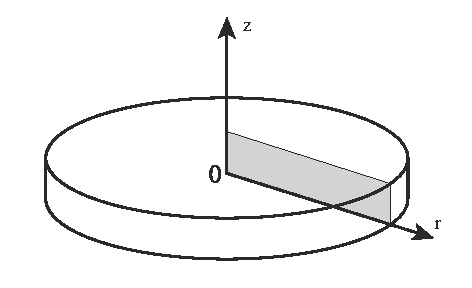
\includegraphics[width=80mm]{images/disc.pdf}
\end{figure}

I tried solving an example of examining the time history of the temperature distribution when the disk was cooled from the surroundings, which is listed in the book "Structural analysis example using finite element method". We verified the accuracy of the program by solving this. The outline of the problem is as follows.
%
For a disk with a radius of 1 m and a thickness of 0.1 m in the initial state t = 0, set the boundary condition with the whole being 500 ° C., with t> 0 and the circumference at 0 ° C. Physical properties of the disk are as iron,
%
\begin{itemize}
\item Thermal conductivity ($\alpha$): \SI{48.0}{ \watt /(\meter K)}
\item Specific heat ($c$): \SI{480}{\joule /(\kilogram C)}
\item Density ($\rho$): \num{7.86e3}\SI{}{\kilogram / \meter ^3}
\end{itemize}
%
As shown in Fig. The time history of temperature in such a thermal diffusion problem is exact solution as follows.

\begin{equation}
T=T_0\sum_{n=1}^{\infty} A_n J_0\left(b_n\frac{r}{a}\right)e^{-p_n t}
\end{equation}

However, a: radius of disk, $T_0$: initial temperature, $J_0$: 0 Bessel function of the following,: root of Bessel function of 0th order, $J_1$: 1st order Bessel function
%
\begin{align}
A_n&=\frac{2}{\beta_n J_1(\beta_n)}\\
p_n&=\frac{\lambda}{c\rho}\frac{\beta_n^2}{a^2}.
\end{align}
%
Well, we will analyze this by the finite element method. Analysis was carried out only in the two-dimensional region of the cross section as shown below using axial symmetry.



The interpolation function is used as a triangle primary element, the time integration is used as the time step $dt=1$, and the Crank-Nicolson method is used. The finite element method solution of a cross section at a certain time is as follows.
%file: disc_fem_solution.jpg
Comparison of the exact solution of the temperature distribution after 2 hours and the finite element method solution is as follows
%file: disc_heat.jpg


\if0
& marker (It turns out that finite element method solution fits exact solution);
\section{What I referred to}
\subsection{Books}
| (<a href = "http: //www.amazon.co.jp/gp/product/4781909116? ie = UTF 8 | Fumio Kikuchi |
| Introduction to Finite Element Method of Flow and Heat Conduction | Motoko Yagawa |
| Structural analysis case examples by finite element method From basic problem to practical level problem | Shiratori Masaki, Miyoshi Toshiaki |
\subsection{Links}
: University of Tokyo School of Foundation Sciences, Hisada, Sugiura Laboratory, Professor Watanabe's lecture material | http: //www.sml.k.u-tokyo.ac.jp/members/nabe/
: Heat conduction (Wikipedia) | & link (heat conduction, http: //en. Wikipedia.org/ wiki / heat conduction);
: Thermal conductivity (Wikipedia) | & link (Thermal conductivity, http://en.wikipedia.org/wiki/ Thermal conductivity);

RIGHT: Made by '' 'Nobuyuki UMETANI' '' Umetsan Nobuyuki
RIGHT:
\fi

\end{document}
